\documentclass[a4paper,14pt]{extarticle}
\usepackage[utf8]{inputenc}
\usepackage[english,russian]{babel}

\usepackage{amsthm}
\usepackage{graphicx}
\usepackage{caption}
\usepackage{amssymb}
\usepackage{amsmath}
\usepackage{mathrsfs}
\usepackage{euscript}
\usepackage{graphicx}
\usepackage{subfig}
\usepackage{caption}
\usepackage{color}
\usepackage{bm}
\usepackage{tabularx}
\usepackage{adjustbox}


\usepackage[toc,page]{appendix}

\usepackage{comment}
\usepackage{rotating}

\DeclareMathOperator*{\argmax}{arg\,max}
\DeclareMathOperator*{\argmin}{arg\,min}

\newtheorem{theorem}{Теорема}
\newtheorem{lemma}[theorem]{Лемма}
\newtheorem{corollary}{Следствие}[theorem]
\newtheorem{definition}{Определение}[section]
\newtheorem{example}{Пример}

\numberwithin{equation}{section}

\newcommand*{\No}{No.}

\begin{document}
	\section{Введение}
	В работе рассматривается задача классификации временных рядов в задаче распознавания действий человека по временным рядам, порождаемым датчиками носимых устройств, например, с акселерометра, гироскопа, альтиметра смартфонов или умных браслетов. Существует несколько подходов к классификации временных рядов: среди них можно выделить машины опорных векторов [1, 2], рекурентные [3] и глубокие [4] нейронные сети или решающие деревья. Классификация временных рядов является частным случаем классификации объектов сложной структуры. Из-за того, что подобные задачи возникают во многих областях, например, в обработке сигналов, биологии, финансах, метеорологии, существует довольно много техник ее решения.
	В нашей работе нас интересует решение задачи классификации временных рядов путем построения промежуточного признакового пространства [5]. Этот метод применим не только к задаче классификации рядов с носимых устройств, так как к объектам сложной структуры можно свести соответствующие ряды из других задач. В общем случае подход с промежуточным признаковым пространством разделим на два этапа.
	\begin{itemize}
		\item На первом этапе для сегментов временных рядов, которые выступают в роли объектов (которые, вообще говоря, могут быть различной длины и даже частоты дискретизации) вычисляются некоторые статистики или добываются некоторые экспертные оценки. В результате на каждый объект мы имеем некоторый набор численных показателей.
		\item 	Над вторичным пространством этих показателей (то есть преобразованными объектами) работает некоторый алгоритм классификации (например ...), который обучается на "вторичной"выборке.
		Эти этапы зависимы, так как классификатор, используемый во втором этапе может потребовать от обучающей выборки выполнимость некоторых гипотез и, в частности, гипотезы простоты выборки, что может быть обепечено только корректным первым этапом. Выполнимость гипотезы простоты выборки, находящейся в промежуточном пространстве, необходима для корректной работы алгоритмов классификации.
	\end{itemize}
	
	
	\section*{Постановка задачи}
	Рассмотривается некоторый временной ряд, то есть функцию определенную на множестве временных меток. 
	\begin{equation}
		S:T\rightarrow\mathbb{R},
	\end{equation}
	где $T = \left\lbrace t_0,t_0+d,t_0+2d,\dots\right\rbrace, \left|T\right|< \infty$.
	
	Зададается некоторая ширина сегмента $n \in \mathbb{N}$, тогда объектом $\mathbf{x}_i$ называется набор:
	\begin{equation}
	\mathbf{x}_i = [(S(t_i),S(t_i - d),S(t_i-2d),\dots,S(t_i - (n-1)d))]^T,
	\end{equation}
	где $\mathbf{x}_i \in X\equiv\mathbb{R}^n$.
	
	Необходимо восстановить зависимость $y = f(\mathbf{x})$, $f:X\rightarrow Y$. Если $Y = \left\lbrace1,2,\dots,K \right\rbrace $, то решается задача многоклассовой классификации. Если же $Y = \mathbb{R}$, то решается задачи регрессии. Для этого задается обучающая выборка
	\begin{equation}
	\mathcal{D} = \left\lbrace (\mathbf{x}_i,y_i)\right\rbrace ^l_{i=1}
	\end{equation}
	где $\left\lbrace \mathbf{x}_i\right\rbrace $ --- набор сегментов данных акселерометра, ${y_i}$ --- метки классов движения в задаче классификации, либо действительное число в задаче регрессии.
	
	Вводятся функции потерь:
	\begin{equation}
	L(f(\mathbf{x}_i),y_i) = \sum_{i=1}^{l}\sum_{k=1}^{K}[y_i = k]\log P(y_i = k|\mathbf{x}_i,\theta)
	\end{equation}  
	для задачи классификации. 
	\begin{equation}
	L(f(\mathbf{x}_i),y_i) = \sum_{i=1}^{l}(y_i - f(\mathbf{x}_i,\theta))^2
	\end{equation}
	для задачи регрессии.
	Таким образом решается задача оптимизации
	\begin{equation}
	\hat{\theta} = \argmin_{\theta \in \Theta} \sum_{i=1}^{l}L(f(\mathbf{x}_i,\theta),y_i)
	\end{equation}
	
	
	\subsection*{Комбинированное признаковое описание}
	Пусть $H$ --- множество функций вида $h : X \rightarrow \mathbb{R}^m$, где $m = m(h)$, то есть это множество отображений пространства объектов сложной структуры в пространство действительных чисел некоторой размерности (для каждой функции размерность может быть своя). В $H$ могут лежать например
	\begin{itemize}
		\item Множество моделей локальной аппроксимации сигнала
		\item Множество статистик
		\item Множество экспертных оценок каждого из сложных объектов
	\end{itemize}
	Возьмем конечный поднабор этих функций
	\begin{equation}
	\mathbf{h} = [h_1,h_2,\dots,h_k], \left\lbrace h_1,h_2,\dots,h_k \right\rbrace \subset H
	\end{equation}
	Обозначим сумму размерностей образов функций из набора как
	\begin{equation}
		n_\mathbf{h} = dim(Im(h_1))+dim(Im(h_2))+\dots+dim(Im(h_k))
	\end{equation}
	Тогда h индуцирует отображение  $h : X \rightarrow Z \subset R^{n_\mathbf{h}}$ , причем в векторах образа первые $dim(Im(h1))$ компонент соответствуют образу $h_1$, следующие $dim(Im(h_2))$ соответствуют $h_2$ и так далее. $Z$ называется признаковым пространством объектов сложной структуры $X$. Тогда, находится $f$ в семействе суперпозиций $a(h(\cdot), \gamma)$, где
	\begin{equation}
	T\rightarrow X\rightarrow Z \rightarrow Y
	\end{equation}
	\begin{itemize}
		\item h --- это признаковое отображение
		\item $a(\cdot,\gamma)$ — параметрическое отображение $Z$ в $Y$, которое соответствует некоторому алгоритму машинного обучения, параметризованного вектором гиперпараметров $\gamma$.
	\end{itemize}
В таком подходе функция потерь теперь определена на отображении $a$, то есть
\begin{equation}
L(f(x),y) = L(a(h(x),\gamma),y)
\end{equation}
Итак, задача решается следующим образом: 
\begin{itemize}
	\item Поиск и вычисление отображения $Z = {\mathbf{h(x_i)}}^l_{i=1}$ путем минимизации функционалов ошибок для каждой модели локальной аппроксимации и поиска оптимальных параметров
	\begin{equation}
	\argmin_{\mathbf{w} \in W} L_{\mathbf{h}}(X,\mathbf{w}) =  	\argmin_{\mathbf{w} \in W} \sum_{i=1}^{l}\sum_{k=1}^{n}\left\| \mathbf{h}(\mathbf{w},x_i)-x_i\right\|_2^2 
	\end{equation}
	\item Оптимизация функции ошибки обобщенной линейной модели, которая в качестве обучающей выборки имеет $(Z, y)$.
	\begin{equation*}
	\argmin_{\theta \in \Theta} L_a(Z,y,\theta) = \argmin_{\theta \in \Theta} -\sum_{i=1}^{l}\sum_{k=1}^K[y_i = k]\log P(y_i=k|z_i,\theta)
	\end{equation*}
	Основное допущение, принимаемое в данном методе является допущение о том, что выборка в признаковом пространстве объектов является простой. В данной работе мы рассматриваем, для каких признаковых пространств это допущение справедливо, а также предлагаем способы построения таких выборок.
	
\end{itemize}

\subsection*{Введение понятия сложности датасета}
Для задачи прогнозирования предполагается использование линейных и обобщенно линейных моделей, так как они не требуют больших вычислительных ресурсов. Для того, чтобы данные модели работали корректно, нужно потребовать некоторые условия для датасета. Самым простым требованием является то, что датасет должен был быть поражден одной линейной или обобщенной линейной моделью. Однако такое требование слишком строгое, а также один и тот же датасет может быть поражден разными моделями.  В качестве примера можно привести выборку со смесью двух нормальных распределений, где в первом случае их просто получили смесью двух выборок, а во втором она пораждалась из одного распределения (распределение бернулли и два нормальных распределения).

Рассмотрим регрессионое уравнение 
\begin{equation}
y = b+w\cdot x+\varepsilon
\end{equation}
Для задачи регрессии существует теорема Гаусса-Маркова, которая перечисляет условия, когда линейная регрессия оптимальна. 
\begin{theorem}[Гаусс, Марков] Рассмотрим следующие предположения
\begin{itemize}
	\item $y_t = b+w\cdot x_t+\varepsilon_t$ --- спецификация модели, отражающая наше представление о механизме зависимости.
	\item $X_t$ --- детерминированная экзогенная переменная. Случайный член должен быть распределен независимо от объясняющей переменной.
	\item $M(\varepsilon) = 0$, то есть случайный член не должен иметь систематического смещения. Это условие всегда можно выполнить, если модель включает свободный член, который будет учитывать любую систематическую  тенденцию. Можно считать это условие выполняющимся автоматически.
	\item   $D(\varepsilon) = M(\varepsilon^2) - M(\varepsilon)^2 = M(\varepsilon^2) = \sigma^2 = Const$ для всех наблюдений. Условие независимости дисперсии от номера наблюдений называют гомоскедастичностью. Случай не выполнения условия гомоскедастичности называют гетероскедастичностью --- $M(\varepsilon^2) = \sigma^2 \neq Const$.
	\item $cov(\varepsilon_i, \varepsilon_j) = M(\varepsilon_i \varepsilon_j) - M(\varepsilon_i)M(\varepsilon_j) = M(\varepsilon_i \varepsilon_j) = 0$. Предполагается отсутствие систематической связи между значениями  для разных наблюдений. Случайные члены должны быть независимыми. В случае, когда это свойство нарушается (временные ряды), говорят об автокорреляции $M(\varepsilon_i \varepsilon_j) \neq 0$.
\end{itemize}
в данных предположениях оценки параметров регрессии, полученные МНК, имеют наименьшую дисперсию в классе всех линейных несмещенных оценок.
\end{theorem}

К сожалению, проверить данные предположения на практике невозможно, так как имея только датасет, нет возможности оценивать мат. ожтдание и дисперсию $\varepsilon_i$

Поэтому требуется разработать метод, как порождать датасет, который будет хорошо описываться линейными и обобщенно линейными моделями, а также ввести понятие сложности датасета.

Для введения понятия сложности приведем теорему об универсальной апроксимации.
\begin{theorem}[Цыбенко, 1989]
	Пусть $\phi$ --- ограниченная, не постоянная монотонно возрастающая непрерывная функция. Введем в рассмотрение $I_{m_0}$--- $m_0$-мерный единичный гиперкуб $[0,1]^{m_0}$. Пусть пространство непрерывных на  $I_{m_0}$ функций обозначается символом $C(I_{m_0})$. Тогда для любой функции $f \in C(I_{m_0})$ существует такое целое число $m_1$  и множество действительных констант $a_i,b_i,w_i$ где $i=1,\dots,m_1$,$j =  1,\dots,m_0$, что
	\begin{equation}
	F(x_1,\dots,\xi_{m_0}) = \sum_{i=1}^{m_1}a_i\phi\left(\sum_{j=1}^{m_0}w_{ij}x_j+b_i\right)
	\end{equation}
	является реализацией аппроксимации функции $f(\cdot)$, т.е.
	\begin{equation}
	\left\| F(x_1,\dots,x_{m_0}) - f(x_1,\dots,x_{m_0}) \right\| < \varepsilon
	\end{equation}
	 для всех $x_1,x_2,\dots,x_{m_0}$ принадлежащих входному пространству.
	
	
	
\end{theorem}

Благодаря данной теореме мы можем аппроксимировать функцию используя только два слоя нейросети. Заметим, что на последнем слое нейросети используется либо обобщенно линейная, либо просто линейная модель, а значит в случае хорошей аппроксимации на скрытом слое находится представление исходного датасета, которое хорошо анализируется линейной или обобщенно линейной моделью. Также стоит заметить, что при увеличении нейронов на скрытом слое ошибка будет падать, но это будет вести к переобучению. Данные рассуждения приводят на к следующему определению сложности.

\begin{definition}
	\label{def1}
	Определим сложность датасета как минимальное количество нейронов на скрытом слое двухслойной полносвязной нейронной сети, аппроксимирующая с заданым качеством $L^*$.
	\begin{equation}
	Comp_{L^*}(\mathcal{D}) = \min (N|L = L^*)\text{|neurons in the hidden layer|}
	\end{equation}
\end{definition}
Для того, чтобы показать, что наше определение сложности датасета корректно, строится графики зависимости дисперсии ошибки и коэффициент детерминации от количества нейронов, чтобы показать, что определенное количество нейронов на скрытом слое достаточно, и, начиная с некоторого, добавление новых нейронов является избыточным. 

Корректное определение сложности датасета дает возможность численно оценивать, а также искать способы как можно упрощать датасеты для более качественной обработки.

\section{Постановка эксперимента}
Для того, чтобы показать, что определение \ref{def1} корректно для линейной регрессии, требуется проверить требования теоремы Гаусса-Маркова. Однако это сделать невозможно, так как нам представлен только один датасет. Поэтому в данной статье будут проверяться следующие параметры: корреляция ошибок, дисперсия ошибок, среднее ошибок и коэффициент детерминации $R^2$.  


В вычислительном эксперименте использовались следующее семейство моделей локальной аппроксимации:
\begin{itemize}
	\item SSA с параметром 5
	\item SSA с параметром 10
	\item AR-авторегрессия с параметром 2
	\item AR-авторегрессия с параметром 4
%	\item FFT с 2 старшими частотами
%	\item FFT с 5 старшими частотами
%	\item SEMOR с профилем ходьбы
%	\item SEMOR с профилем бега
%	\item SEMOR с профилем ходьбы вверх по лестнице
%	\item SEMOR с профилем ходьбы вниз по лестнице
\end{itemize}

\begin{figure}[h!]
	
	\begin{minipage}{0.5\linewidth}
		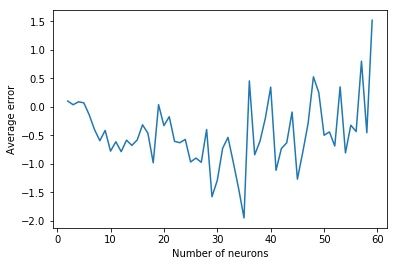
\includegraphics[width=1\linewidth]{avg_error.jpg} 
	\end{minipage}
	\hfill
	\begin{minipage}{0.5\linewidth}
		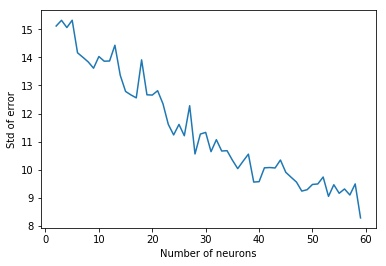
\includegraphics[width=1\linewidth]{std_error.jpg}
	\end{minipage}\\
	\begin{minipage}{0.5\linewidth}
		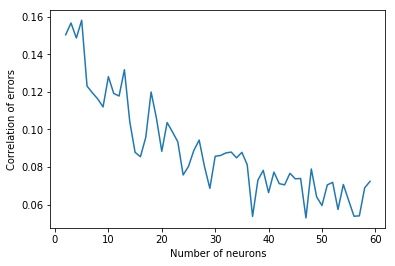
\includegraphics[width=1\linewidth]{corr_err.jpg}
	\end{minipage}
	\hfill
	\begin{minipage}{0.5\linewidth}
		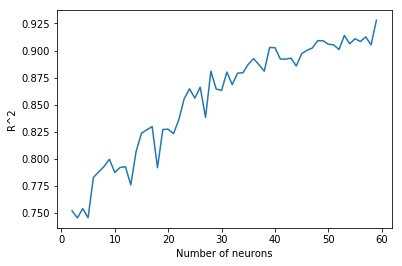
\includegraphics[width=1\linewidth]{R^2.jpg}
	\end{minipage}\\
	
	\caption{a) среднее значение ошибки б) дисперсия ошибки
		в) корреляция ошибки г) коэффициент детерминации}
\end{figure}



В качестве обобщенно линейной модели будет использовать модель логистической регрессии:
\begin{equation}
f(z) = \frac{1}{1+e^{-z}}, z = \mathbf{w}^T\mathbf{x} = w_0 + w_1 x^{(i)}_1 + \dots + w_n x^{(i)}_n
\end{equation}
Функция ошибки --- минус логарифм правдоподобия.
\begin{equation*}
Q = -\ln L(w) = \sum_{i=1}^m \log \mathbb{P}\{y=y^{(i)} \mid x=x^{(i)}\}
= 
\end{equation*}
$$=\sum_{i=1}^m y^{(i)} \ln f(\mathbf{w}^T x^{(i)}) + (1 - y^{(i)}) \ln (1 - f(\mathbf{w}^T x^{(i)}))$$
В качестве аналога отклонения $\hat{y}_i - y_i$ будем использовать $ y^{(i)}\ln p_i + (1-y^{(i)})\ln(1-p_i) = y^{(i)} \ln f(\mathbf{w}^T x^{(i)}) + (1 - y^{(i)}) \ln (1 - f(\mathbf{w}^T x^{(i)}))$. Построим также графики корреляции, дисперсии, среднего ошибки и псевдо-$R^2$.

\begin{figure}[h!]
	
	\begin{minipage}{0.5\linewidth}
		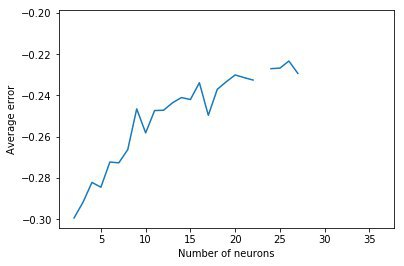
\includegraphics[width=1\linewidth]{avgerrlogreg.jpg} 
	\end{minipage}
	\hfill
	\begin{minipage}{0.5\linewidth}
		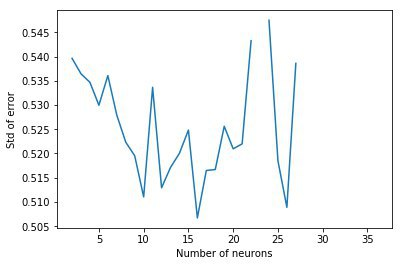
\includegraphics[width=1\linewidth]{stdlogreg.jpg}
	\end{minipage}\\
\end{figure}
Для оценки разброса $R^2$ и pseudo-$R^2$ использовалось сэмплирование по подвыборкам
\begin{figure}[h!]
	
	\begin{minipage}{0.5\linewidth}
		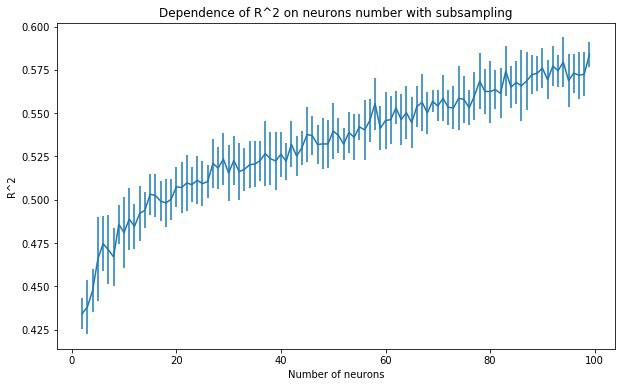
\includegraphics[width=1\linewidth]{goodR^2.jpg} 
	\end{minipage}
	\hfill
	\begin{minipage}{0.5\linewidth}
		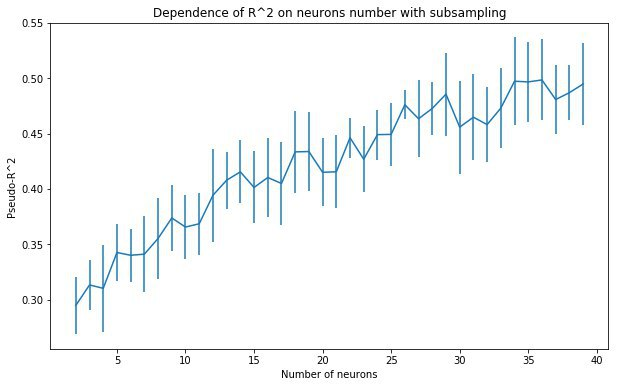
\includegraphics[width=1\linewidth]{pseudoR^2.jpg}
	\end{minipage}\\
\end{figure}
	

	
\end{document}